\chapter{Appendix}\label{ch:appendix}
\renewcommand{\thefigure}{A\arabic{figure}}
\renewcommand{\thetable}{A\arabic{table}}
\renewcommand{\thelstlisting}{A\arabic{lstlisting}}
\renewcommand{\thesection}{A\arabic{section}}

\section{Expression Rewrite Rules}\label{app_rewrite_rules}

In \cref{tab:all_rewrite_rules}, we list the complete set of expression rewrite rules we implemented in the optimizer, grouped by pass.
We characterize each rule by its pass assignment, scope (filter-only or both filters and paint/layout properties), type (pure, MIR-aware, or stats-driven), and a brief description of the pattern it matches and the rewrite it produces.

\begin{longtblr}[
  caption = {Complete list of expression rewrite rules},
  label = {tab:all_rewrite_rules},
]{
  colspec = {r l l l X},
  row{1} = {font=\bfseries},
  rowhead = 1,
}
\toprule
\# & Pass & Scope & Type & Description \\
\midrule
% Expression Kind
1 & Expr.\ kind & both & MIR & Negate comparison: \texttt{[\mlop{"!"},[\mlop{op},a,b]]} $\to$ \texttt{[\mlop{neg(op)},a,b]} when negated operator exists \\
\midrule
% Constant Fold
2 & Const.\ fold & both & pure & Boolean algebra: fold \mlop{any}/ \mlop{all} with literal operands; absorb \mlval{true} from \mlop{all}, \mlval{false} from \mlop{any} \\
3 & Const.\ fold & both & pure & Fold negation: \texttt{[\mlop{"!"}, \mlval{true}]} $\to$ \mlval{false} \\
4 & Const.\ fold & both & pure & Fold comparisons (\mlop{==}, \mlop{!=}, \texttt{<}, etc.) with two literal operands \\
5 & Const.\ fold & both & MIR & Evaluate pure operators when all arguments are literals \\
6 & Const.\ fold & both & pure & Algebraic identity: \texttt{x \^{} \mlval{0}} $\to$ \mlval{1} \\
7 & Const.\ fold & both & pure & Strip redundant \mlop{typeof} guards from migrated filters \\
8 & Const.\ fold & both & pure & Resolve \mlop{case} arms with known boolean conditions \\
9 & Const.\ fold & both & pure & Resolve \mlop{match} when input is a known literal \\
10 & Const.\ fold & both & pure & \acs{SCCP}: substitute equality bindings into \mlop{case} arm bodies \\
11 & Const.\ fold & both & pure & \acs{SCCP}: substitute equality bindings into \mlop{match} arm bodies \\
12 & Const.\ fold & both & pure & Detect contradictory \mlop{==}/ \mlop{!=} predicates in \mlop{all} $\to$ \mlval{false} \\
13 & Const.\ fold & both & pure & Substitute equality bindings into sibling predicates in \mlop{all} \\
14 & Const.\ fold & both & pure & Subsume weaker range bounds: keep tighter of two bounds on same variable \\
15 & Const.\ fold & both & pure & Remove \mlop{has} subsumed by comparison on the same property \\
16 & Const.\ fold & both & pure & Boolean absorption: \texttt{[\mlop{"all"},A,[\mlop{"any"},A,\ldots]]} $\to$ \texttt{[\mlop{"all"},A]} \\
17 & Const.\ fold & both & pure & Remove redundant type coercions on already-typed values \\
18 & Const.\ fold & both & pure & Strip explicit \texttt{[\mlop{"properties"}]} argument from \mlop{get}/ \mlop{has} \\
\midrule
% Constant Fold Stats
19 & Fold (stats) & filter & stats & Fold \texttt{[\mlop{"has"},p]} $\to$ true/false when stats confirm property presence \\
20 & Fold (stats) & both & stats & Fold \texttt{[\mlop{"get"},p]} to literal when property has a single value \\
21 & Fold (stats) & filter & stats & Fold geometry-type comparison from observed types in tile statistics \\
22 & Fold (stats) & both & stats & Fold comparison to true/false when value distribution proves constant result \\
23 & Fold (stats) & both & stats & Prune impossible labels from \mlop{in} expression using value statistics \\
24 & Fold (stats) & both & stats & Prune \mlop{match} arms whose labels never appear in property value counts \\
25 & Fold (stats) & both & stats & Reorder \mlop{match} arms by descending value frequency \\
26 & Fold (stats) & both & stats & Fold \mlop{coalesce} when \mlop{get} arm is always or never present \\
27 & Fold (stats) & both & stats & Prune unreachable \mlop{interpolate}/ \mlop{step} stops outside observed data range \\
\midrule
% Simplify Expressions
28 & Simplify & both & pure & Factor common operands:\newline \texttt{[\mlop{"any"},[\mlop{"all"},A,B],[\mlop{"all"},A,C]]} $\to$ \texttt{[\mlop{"all"},A,[\mlop{"any"},B,C]]} \\
29 & Simplify & both & pure & Canonicalise \texttt{[\mlop{"exponential"},\mlval{1}]} $\to$ \texttt{[\mlop{"linear"}]} in interpolate curves \\
30 & Simplify & both & pure & Collapse \mlop{interpolate}/ \mlop{step} when all output values are structurally equal \\
31 & Simplify & both & pure & Merge \mlop{match} arms with identical outputs; drop arms that equal the fallback \\
32 & Simplify & both & pure & Strip \mlop{coalesce} wrapper from comparison when default fails anyway \\
33 & Simplify & both & pure & Strip \mlop{coalesce} from \mlop{match} input when default not in any label \\
34 & Simplify & both & pure & Strip \mlop{coalesce} from \mlop{in} needle when default not in haystack \\
35 & Simplify & both & pure & Rewrite single-arm boolean \mlop{match} to \mlop{in}/ \mlop{==}/ \mlop{!=} \\
36 & Simplify & both & pure & Rewrite \texttt{[\mlop{"any"},[\mlop{"=="},x,a],\ldots]} $\to$ \texttt{[\mlop{"in"},x,[\ldots]]} \\
37 & Simplify & both & pure & Flatten nested \mlop{case}: inline the fallback's arms \\
38 & Simplify & both & pure & Remove trailing \mlop{case} arms whose output equals the fallback \\
39 & Simplify & both & pure & Rewrite \mlop{case} to \mlop{match} for $\mathcal{O}(1)$ dispatch when all arms test equality on the same expression \\
40 & Simplify & both & pure & Simplify \mlop{coalesce}: remove null literals, truncate after first non-null literal \\
41 & Simplify & both & pure & Flatten nested \mlop{coalesce} expressions \\
42 & Simplify & both & pure & Flatten nested \mlop{all}/ \mlop{any} operators \\
43 & Simplify & both & pure & De Morgan's laws: \texttt{[\mlop{"!"},[\mlop{"any"},A,B]]} $\to$ \texttt{[\mlop{"all"},[\mlop{"!"},A],[\mlop{"!"},B]]} \\
44 & Simplify & both & pure & Single-element \mlop{in} $\to$ \mlop{==} \\
45 & Simplify & both & pure & Merge adjacent \mlop{in} expressions on the same variable inside \mlop{any} \\
46 & Simplify & both & pure & Inline single-use \mlop{let}/ \mlop{var} bindings \\
\midrule
% Selectivity
47 & Selectivity & both & stats & Reorder \mlop{any}/ \mlop{all} operands by estimated selectivity for short-circuit evaluation \\
\bottomrule
\end{longtblr}
\clearpage

\section{MapLibre GL-JS Reference Excerpts}

The two render-pass loops the painter runs over \texttt{layerIds} (the opaque pass top-to-bottom and the translucent pass bottom-to-top) are the basis for the layer-merging savings discussed in \cref{sub:structural_optimizations}.
Every layer eliminated by a merge shortens \texttt{layerIds} and removes one texttt{renderLayer} dispatch from each pass.

\begin{lstlisting}[language=TypeScript,caption={MapLibre GL-JS painter render loop (\texttt{src/render/painter.ts})},label=lst:painter_loop]
// opaque pass (top-to-bottom)
for (this.currentLayer = layerIds.length - 1;
     this.currentLayer >= 0; this.currentLayer--) {
    const layer = this.style._layers[layerIds[this.currentLayer]];
    const tileManager = tileManagers[layer.source];
    const coords = coordsAscending[layer.source];
    this._renderTileClippingMasks(layer, coords, false);
    this.renderLayer(this, tileManager, layer, coords, renderOptions);
}

// translucent pass (bottom-to-top)
for (this.currentLayer = 0;
     this.currentLayer < layerIds.length; this.currentLayer++) {
    const layer = this.style._layers[layerIds[this.currentLayer]];
    const tileManager = tileManagers[layer.source];
    // ...
    this.renderLayer(this, tileManager, layer, coords, renderOptions);
}
\end{lstlisting}

\Cref{lst:placement} reproduces the per-layer placement loop that justifies the exclusion of symbol layers from the merge candidate set in \cref{sub:structural_optimizations}, where \stepcirc{1} constructs a fresh \texttt{LayerPlacement} when a symbol layer's placement begins and \stepcirc{2} tears it down before the next layer starts.
This means that two symbol layers fused into one would interleave their symbols within a single \texttt{LayerPlacement} and alter collision outcomes.

\begin{lstlisting}[
	language=TypeScript,
	escapeinside={(*@}{@*)},
	caption={MapLibre GL-JS  symbol placement (\texttt{src/style/pauseable\_placement.ts})},
	label=lst:placement]
while (this._currentPlacementIndex >= 0) {
    const layerId = order[this._currentPlacementIndex];
    const layer = layers[layerId];
    const placementZoom = this.placement.collisionIndex.transform.zoom;
    if (isSymbolStyleLayer(layer) && layer.layout &&
        (!layer.minzoom || layer.minzoom <= placementZoom) &&
        (!layer.maxzoom || layer.maxzoom > placementZoom)) {

        if (!this._inProgressLayer) {
          (*@\stepcirc{1}@*) this._inProgressLayer = new LayerPlacement(layer);
        }
        const pausePlacement = this._inProgressLayer.continuePlacement(
            layerTiles[layer.source], this.placement,
            this._showCollisionBoxes, layer, shouldPausePlacement
        );
        if (pausePlacement) return;
      (*@\stepcirc{2}@*) delete this._inProgressLayer;
    }
    this._currentPlacementIndex--;
}
\end{lstlisting}

\Cref{lst:bucket_populate} reproduces the \texttt{FillBucket.populate} method, which witnesses the filter-first evaluation order on which the filter-to-property constant-propagation pass in \cref{sub:structural_optimizations} depends.
In it, \stepcirc{1} rejects a feature before any paint or layout expression is evaluated, so any equality constraint extracted from a layer's filter is guaranteed to hold for every feature that reaches \stepcirc{2}.

\begin{lstlisting}[
	language=TypeScript,
	escapeinside={(*@}{@*)},
	caption={MapLibre GL-JS bucket populate method showing filter-first evaluation (\texttt{src/data/bucket/fill\_bucket.ts})},
	label=lst:bucket_populate]
for (const {feature, id, index, sourceLayerIndex} of features) {
    const needGeometry = this.layers[0]._featureFilter.needGeometry;
    const evaluationFeature = toEvaluationFeature(feature, needGeometry);

    (*@\stepcirc{1}@*) if (!this.layers[0]._featureFilter.filter(
        new EvaluationParameters(this.zoom), evaluationFeature, canonical
    )) continue;  // feature rejected: no paint evaluation occurs

    // Only reached for features that passed the filter:
    const bucketFeature: BucketFeature = {
        id, properties: feature.properties, type: feature.type,
        sourceLayerIndex, index,
        geometry: needGeometry ? evaluationFeature.geometry
                               : loadGeometry(feature),
        patterns: {}, sortKey
    };
    (*@\stepcirc{2}@*) bucketFeatures.push(bucketFeature);
}
\end{lstlisting}
\clearpage

\section{Camera Animation Patterns}\label{app:animation_patterns}
\Cref{fig:app_animation_patterns} visualizes the five animation patterns.

\begin{figure}[htbp]
	\centering
	\tikzset{
		framebox/.style={draw=gray, line width=0.3pt, fill=white},
		crosshair/.style={draw=gray!60, line width=0.2pt},
		trajpath/.style={draw=cvdblue, line width=0.7pt,
			postaction={decorate, decoration={markings,
					mark=at position 0.5 with {
						\arrow{Stealth[length=0.9mm, width=0.55mm]}
					}
			}}
		},
		trajdot/.style={circle, fill=cvdblue, inner sep=0pt, minimum size=2.6pt, draw=none},
		trajstart/.style={circle, draw=cvdblue, line width=0.8pt, fill=white,
			inner sep=0pt, minimum size=4.6pt},
		trajend/.style={rectangle, fill=cvdblue, inner sep=0pt, minimum size=3.8pt, draw=none},
		stationary/.style={circle, fill=cvdvermillion, draw=darkgray, line width=0.3pt,
			inner sep=0pt, minimum size=4pt},
		statlabel/.style={font=\tiny, text=darkgray},
		bar/.style={fill=cvdblue, draw=none},
		constline/.style={draw=darkgray, line width=0.4pt, dashed},
		axislabel/.style={font=\tiny, text=darkgray},
		striplabel/.style={font=\fontsize{3pt}{3.6pt}\selectfont, text=darkgray},
		bearingarrow/.style={-{Stealth[length=1.4mm, width=1.0mm]}, draw=cvdblue, line width=0.45pt},
	}
	% z-strip geometry: single source of truth for the z->y mapping used
	% by bar tops, numeric labels and dashed constant lines across all panels.
	% Strip has total height \striph=0.5; drawable area is [\zPad, \striph-\zPad].
	% \zTop{z} linearly maps zoom z in [1,24] to that drawable area.
	\providecommand{\zPad}{0.04}%
	\providecommand{\zTop}[1]{\zPad + ((#1-1)/23)*(\striph-2*\zPad)}%

	%% ── (a) zigzag ────────────────────────────────────────────────────────────
	\begin{subfigure}[t]{0.31\linewidth}
		\centering\vspace{0pt}%
		\resizebox{\linewidth}{!}{%
			\begin{tikzpicture}
				\def\mapsize{1.8} \def\stripw{1.8} \def\striph{0.5}
				\def\stripx{0} \def\zstripy{0.65} \def\bstripy{0}
				\def\mapy{1.35}
				\def\mapcx{0.9} \def\mapcy{2.25} \def\trajscale{0.78}

				\draw[framebox] (0, \mapy) rectangle (\mapsize, \mapy+\mapsize);
				\draw[crosshair] (0, \mapcy) -- (\mapsize, \mapcy);
				\draw[crosshair] (\mapcx, \mapy) -- (\mapcx, \mapy+\mapsize);
				\node[axislabel, anchor=north] at (\mapcx, \mapy-0.1) {$\mathrm{lng}$};
				\node[axislabel] at (-0.25, \mapcy) {$\mathrm{xy}$};
				\foreach \i/\nx/\ny in {%
					0/0.125/0.125, 1/0.25/-0.25, 2/0.375/0.375, 3/0.5/-0.5,%
					4/0.625/0.625, 5/0.75/-0.75, 6/0.875/0.875, 7/1.0/-1.0} {
					\coordinate (zz\i) at ({\mapcx + \trajscale*\nx}, {\mapcy + \trajscale*\ny});
				}
				\foreach \a/\b in {0/1,1/2,2/3,3/4,4/5,5/6,6/7} { \draw[trajpath] (zz\a) -- (zz\b); }
				\foreach \i in {0,...,7} { \node[trajdot] at (zz\i) {}; }
				\node[trajstart] at (zz0) {};
				\node[trajend]   at (zz7) {};

				% zoom strip — 8 bars alternating z10/z14
				\draw[framebox] (\stripx, \zstripy) rectangle (\stripx+\stripw, \zstripy+\striph);
				\node[axislabel, anchor=east] at (\stripx-0.04, \zstripy+\striph/2) {$z$};

				\foreach \i/\z in {0/10, 1/14, 2/10, 3/14, 4/10, 5/14, 6/10, 7/14} {
					\pgfmathsetmacro{\bx}{\stripx + (\i+0.5)*\stripw/8 - 0.08}
					\pgfmathsetmacro{\h}{\zTop{\z}}
					\draw[bar] (\bx, \zstripy+\zPad) rectangle (\bx+0.16, \zstripy+\h);
				}
				\pgfmathsetmacro{\hHi}{\zTop{24}}
				\pgfmathsetmacro{\hLo}{\zTop{1}}
				\node[striplabel, anchor=west] at (\stripx+\stripw-0.01, \zstripy+\hHi) {24};
				\node[striplabel, anchor=west] at (\stripx+\stripw-0.01, \zstripy+\hLo) {1};

				% bearing strip — 8 arrows, 0..105
				\draw[framebox] (\stripx, \bstripy) rectangle (\stripx+\stripw, \bstripy+\striph);
				\node[axislabel, anchor=east] at (\stripx-0.04, \bstripy+\striph/2) {$\theta$};
				\foreach \i/\b in {0/0, 1/15, 2/30, 3/45, 4/60, 5/75, 6/90, 7/105} {
					\pgfmathsetmacro{\bcx}{\stripx + (\i+0.5)*\stripw/8}
					\pgfmathsetmacro{\bcy}{\bstripy + \striph/2}
					\pgfmathsetmacro{\dx}{0.13*sin(\b)}
					\pgfmathsetmacro{\dy}{0.13*cos(\b)}
					\draw[bearingarrow] (\bcx, \bcy) -- ($(\bcx, \bcy) + (\dx, \dy)$);
				}
			\end{tikzpicture}%
		}
		\caption{\textbf{Zigzag.} Stresses zoom-triggered layer-visibility changes alongside tile loading.}
		\label{fig:app_anim_zigzag}
	\end{subfigure}
	\hfill
	%% ── (b) spiral ────────────────────────────────────────────────────────────
	\begin{subfigure}[t]{0.31\linewidth}
		\centering\vspace{0pt}%
		\resizebox{\linewidth}{!}{%
			\begin{tikzpicture}
				\def\mapsize{1.8} \def\stripw{1.8} \def\striph{0.5}
				\def\stripx{0} \def\zstripy{0.65} \def\bstripy{0}
				\def\mapy{1.35}
				\def\mapcx{0.9} \def\mapcy{2.25} \def\trajscale{0.78}

				\draw[framebox] (0, \mapy) rectangle (\mapsize, \mapy+\mapsize);
				\draw[crosshair] (0, \mapcy) -- (\mapsize, \mapcy);
				\draw[crosshair] (\mapcx, \mapy) -- (\mapcx, \mapy+\mapsize);
				\node[axislabel, anchor=north] at (\mapcx, \mapy-0.1) {$\mathrm{lng}$};
				\node[axislabel] at (-0.25, \mapcy) {$\mathrm{xy}$};
				\foreach \i in {0,...,11} {
					\pgfmathsetmacro{\ang}{\i*30}
					\coordinate (sp\i) at ({\mapcx + \trajscale*cos(\ang)},
					{\mapcy + \trajscale*sin(\ang)});
				}
				\foreach \a/\b in {0/1,1/2,2/3,3/4,4/5,5/6,6/7,7/8,8/9,9/10,10/11} { \draw[trajpath] (sp\a) -- (sp\b); }
				\foreach \i in {0,...,11} { \node[trajdot] at (sp\i) {}; }
				\node[trajstart] at (sp0)  {};
				\node[trajend]   at (sp11) {};

				% zoom strip — constant z12, 12 bars
				\draw[framebox] (\stripx, \zstripy) rectangle (\stripx+\stripw, \zstripy+\striph);
				\node[axislabel, anchor=east] at (\stripx-0.04, \zstripy+\striph/2) {$z$};
				\pgfmathsetmacro{\hC}{\zTop{12}}
				\foreach \i in {0,...,11} {
					\pgfmathsetmacro{\bw}{0.11}
					\pgfmathsetmacro{\bx}{\stripx + (\i+0.5)*\stripw/12 - \bw/2}
					\draw[bar] (\bx, \zstripy+\zPad) rectangle (\bx+\bw, \zstripy+\hC);
				}
				\pgfmathsetmacro{\hHi}{\zTop{24}}
				\pgfmathsetmacro{\hLo}{\zTop{1}}
				\node[striplabel, anchor=west] at (\stripx+\stripw-0.01, \zstripy+\hHi) {24};
				\node[striplabel, anchor=west] at (\stripx+\stripw-0.01, \zstripy+\hLo) {1};

				% bearing strip — 12 arrows; camera tracks centre, so \b=270-30i (mod 360)
				\draw[framebox] (\stripx, \bstripy) rectangle (\stripx+\stripw, \bstripy+\striph);
				\node[axislabel, anchor=east] at (\stripx-0.04, \bstripy+\striph/2) {$\theta$};
				\foreach \i in {0,...,11} {
					\pgfmathsetmacro{\b}{270-\i*30}
					\pgfmathsetmacro{\bcx}{\stripx + (\i+0.5)*\stripw/12}
					\pgfmathsetmacro{\bcy}{\bstripy + \striph/2}
					\pgfmathsetmacro{\dx}{0.13*sin(\b)}
					\pgfmathsetmacro{\dy}{0.13*cos(\b)}
					\draw[bearingarrow] (\bcx, \bcy) -- ($(\bcx, \bcy) + (\dx, \dy)$);
				}
			\end{tikzpicture}%
		}
		\caption{
\textbf{Spiral.} Camera orbits its target while pointing at it.
This isolates render cost from tile-load cost via a stable tile set.}
		\label{fig:app_anim_spiral}
	\end{subfigure}
	\hfill
	%% ── (c) zoomdrill ─────────────────────────────────────────────────────────
	\begin{subfigure}[t]{0.31\linewidth}
		\centering\vspace{0pt}%
		\resizebox{\linewidth}{!}{%
			\begin{tikzpicture}
				\def\mapsize{1.8} \def\stripw{1.8} \def\striph{0.5}
				\def\stripx{0} \def\zstripy{0.65} \def\bstripy{0}
				\def\mapy{1.35}
				\def\mapcx{0.9} \def\mapcy{2.25}

				\draw[framebox] (0, \mapy) rectangle (\mapsize, \mapy+\mapsize);
				\draw[crosshair] (0, \mapcy) -- (\mapsize, \mapcy);
				\draw[crosshair] (\mapcx, \mapy) -- (\mapcx, \mapy+\mapsize);
				\node[axislabel, anchor=north] at (\mapcx, \mapy-0.1) {$\mathrm{lng}$};
				\node[axislabel] at (-0.25, \mapcy) {$\mathrm{xy}$};
				\node[stationary] at (\mapcx, \mapcy) {};
				\node[statlabel, anchor=north] at (\mapcx, \mapcy-0.15) {stationary};

				% zoom strip — 7 bars z4,8,12,16,12,8,4
				\draw[framebox] (\stripx, \zstripy) rectangle (\stripx+\stripw, \zstripy+\striph);
				\node[axislabel, anchor=east] at (\stripx-0.04, \zstripy+\striph/2) {$z$};

				\foreach \i/\z in {0/4, 1/8, 2/12, 3/16, 4/12, 5/8, 6/4} {
					\pgfmathsetmacro{\bw}{0.17}
					\pgfmathsetmacro{\bx}{\stripx + (\i+0.5)*\stripw/7 - \bw/2}
					\pgfmathsetmacro{\h}{\zTop{\z}}
					\draw[bar] (\bx, \zstripy+\zPad) rectangle (\bx+\bw, \zstripy+\h);
				}
				\pgfmathsetmacro{\hHi}{\zTop{24}}
				\pgfmathsetmacro{\hLo}{\zTop{1}}
				\node[striplabel, anchor=west] at (\stripx+\stripw-0.01, \zstripy+\hHi) {24};
				\node[striplabel, anchor=west] at (\stripx+\stripw-0.01, \zstripy+\hLo) {1};

				% bearing strip — constant 0°, 7 north arrows
				\draw[framebox] (\stripx, \bstripy) rectangle (\stripx+\stripw, \bstripy+\striph);
				\node[axislabel, anchor=east] at (\stripx-0.04, \bstripy+\striph/2) {$\theta$};
				\foreach \i in {0,...,6} {
					\pgfmathsetmacro{\bcx}{\stripx + (\i+0.5)*\stripw/7}
					\pgfmathsetmacro{\bcy}{\bstripy + \striph/2}
					\draw[bearingarrow] (\bcx, \bcy) -- ($(\bcx, \bcy) + (0, 0.13)$);
				}
			\end{tikzpicture}%
		}
		\caption{\textbf{Zoomdrill.} Maximises tile-cache churn.}
		\label{fig:app_anim_zoomdrill}
	\end{subfigure}

	\vspace{0.5em}

	%% ── (d) pansweep ──────────────────────────────────────────────────────────
	\begin{subfigure}[b]{0.31\linewidth}
		\centering\vspace{0pt}%
		\resizebox{\linewidth}{!}{%
			\begin{tikzpicture}
				\def\mapsize{1.8} \def\stripw{1.8} \def\striph{0.5}
				\def\stripx{0} \def\zstripy{0.65} \def\bstripy{0}
				\def\mapy{1.35}
				\def\mapcx{0.9} \def\mapcy{2.25} \def\trajscale{0.78}

				\draw[framebox] (0, \mapy) rectangle (\mapsize, \mapy+\mapsize);
				\draw[crosshair] (0, \mapcy) -- (\mapsize, \mapcy);
				\draw[crosshair] (\mapcx, \mapy) -- (\mapcx, \mapy+\mapsize);
				\node[axislabel, anchor=north] at (\mapcx, \mapy-0.1) {$\mathrm{lng}$};
				\node[axislabel] at (-0.25, \mapcy) {$\mathrm{xy}$};
				\foreach \i/\nx/\ny in {%
					0/-1.0/0.167, 1/-0.667/-0.167, 2/-0.333/0.167,
					3/0.0/-0.167, 4/0.333/0.167,   5/0.667/-0.167} {
					\coordinate (ps\i) at ({\mapcx + \trajscale*\nx},
					{\mapcy + \trajscale*\ny});
				}
				\foreach \a/\b in {0/1,1/2,2/3,3/4,4/5} { \draw[trajpath] (ps\a) -- (ps\b); }
				\foreach \i in {0,...,5} { \node[trajdot] at (ps\i) {}; }
				\node[trajstart] at (ps0) {};
				\node[trajend]   at (ps5) {};

				% zoom strip — constant z12, 6 bars
				\draw[framebox] (\stripx, \zstripy) rectangle (\stripx+\stripw, \zstripy+\striph);
				\node[axislabel, anchor=east] at (\stripx-0.04, \zstripy+\striph/2) {$z$};
				\pgfmathsetmacro{\hC}{\zTop{12}}
				\foreach \i in {0,...,5} {
					\pgfmathsetmacro{\bw}{0.2}
					\pgfmathsetmacro{\bx}{\stripx + (\i+0.5)*\stripw/6 - \bw/2}
					\draw[bar] (\bx, \zstripy+\zPad) rectangle (\bx+\bw, \zstripy+\hC);
				}
				\pgfmathsetmacro{\hHi}{\zTop{24}}
				\pgfmathsetmacro{\hLo}{\zTop{1}}
				\node[striplabel, anchor=west] at (\stripx+\stripw-0.01, \zstripy+\hHi) {24};
				\node[striplabel, anchor=west] at (\stripx+\stripw-0.01, \zstripy+\hLo) {1};

				% bearing strip — constant 0°, 6 north arrows
				\draw[framebox] (\stripx, \bstripy) rectangle (\stripx+\stripw, \bstripy+\striph);
				\node[axislabel, anchor=east] at (\stripx-0.04, \bstripy+\striph/2) {$\theta$};
				\foreach \i in {0,...,5} {
					\pgfmathsetmacro{\bcx}{\stripx + (\i+0.5)*\stripw/6}
					\pgfmathsetmacro{\bcy}{\bstripy + \striph/2}
					\draw[bearingarrow] (\bcx, \bcy) -- ($(\bcx, \bcy) + (0, 0.13)$);
				}
			\end{tikzpicture}%
		}
		\caption{\textbf{Pansweep.} Drives sustained unidirectional (thus predictable) tile cache misses in isolation.}
		\label{fig:app_anim_pansweep}
	\end{subfigure}
	\hfill
	%% ── (e) bearingspin ───────────────────────────────────────────────────────
	\begin{subfigure}[b]{0.31\linewidth}
		\centering\vspace{0pt}%
		\resizebox{\linewidth}{!}{%
			\begin{tikzpicture}
				\def\mapsize{1.8} \def\stripw{1.8} \def\striph{0.5}
				\def\stripx{0} \def\zstripy{0.65} \def\bstripy{0}
				\def\mapy{1.35}
				\def\mapcx{0.9} \def\mapcy{2.25}

				\draw[framebox] (0, \mapy) rectangle (\mapsize, \mapy+\mapsize);
				\draw[crosshair] (0, \mapcy) -- (\mapsize, \mapcy);
				\draw[crosshair] (\mapcx, \mapy) -- (\mapcx, \mapy+\mapsize);
				\node[axislabel, anchor=north] at (\mapcx, \mapy-0.1) {$\mathrm{lng}$};
				\node[axislabel] at (-0.25, \mapcy) {$\mathrm{xy}$};
				\node[stationary] at (\mapcx, \mapcy) {};
				\node[statlabel, anchor=north] at (\mapcx, \mapcy-0.15) {stationary};

				% zoom strip — constant z12, 8 bars
				\draw[framebox] (\stripx, \zstripy) rectangle (\stripx+\stripw, \zstripy+\striph);
				\node[axislabel, anchor=east] at (\stripx-0.04, \zstripy+\striph/2) {$z$};
				\pgfmathsetmacro{\hC}{\zTop{12}}
				\foreach \i in {0,...,7} {
					\pgfmathsetmacro{\bw}{0.16}
					\pgfmathsetmacro{\bx}{\stripx + (\i+0.5)*\stripw/8 - \bw/2}
					\draw[bar] (\bx, \zstripy+\zPad) rectangle (\bx+\bw, \zstripy+\hC);
				}
				\pgfmathsetmacro{\hHi}{\zTop{24}}
				\pgfmathsetmacro{\hLo}{\zTop{1}}
				\node[striplabel, anchor=west] at (\stripx+\stripw-0.01, \zstripy+\hHi) {24};
				\node[striplabel, anchor=west] at (\stripx+\stripw-0.01, \zstripy+\hLo) {1};

				% bearing strip — 8 arrows 0..315
				\draw[framebox] (\stripx, \bstripy) rectangle (\stripx+\stripw, \bstripy+\striph);
				\node[axislabel, anchor=east] at (\stripx-0.04, \bstripy+\striph/2) {$\theta$};
				\foreach \i in {0,...,7} {
					\pgfmathsetmacro{\b}{\i*45}
					\pgfmathsetmacro{\bcx}{\stripx + (\i+0.5)*\stripw/8}
					\pgfmathsetmacro{\bcy}{\bstripy + \striph/2}
					\pgfmathsetmacro{\dx}{0.13*sin(\b)}
					\pgfmathsetmacro{\dy}{0.13*cos(\b)}
					\draw[bearingarrow] (\bcx, \bcy) -- ($(\bcx, \bcy) + (\dx, \dy)$);
				}
			\end{tikzpicture}%
		}
		\caption{\textbf{Bearingspin.} Exercises $\theta$ and high-$\phi$-based \ac{GPU} re-rendering cost without any non-LOD tile loading.}
		\label{fig:app_anim_bearingspin}
	\end{subfigure}
	\hfill
	%% ── (f) DOF matrix + keyframe counts ──────────────────────────────────────
	\begin{subfigure}[b]{0.31\linewidth}
		\centering\vspace{0pt}%
		\begin{tblr}{
				colspec = {l *{5}{c} r},
				rows = {font=\scriptsize},
				row{1} = {font=\scriptsize\bfseries},
				column{1} = {font=\scriptsize},
				colsep = 2.5pt,
				rowsep = 1pt,
			}
			\toprule
			& xy         & z          & $\theta$   & $\phi$     & \# kf \\
			\midrule
			zigzag       & \checkmark & \checkmark & \checkmark & $0^{\circ}$  &  8 \\
			spiral       & \checkmark & --         & \checkmark & $0^{\circ}$  & 12 \\
			zoomdrill    & --         & \checkmark & --         & $0^{\circ}$  &  7 \\
			pansweep     & \checkmark & --         & --         & $0^{\circ}$  &  6 \\
			bearingspin  & --         & --         & \checkmark & $60^{\circ}$ &  8 \\
			\bottomrule
		\end{tblr}
		\caption{
\acs{DOF} matrix, pitch~$\phi$, and keyframe count showing which the most important differientiating factors}
		\label{fig:app_anim_dofs}
	\end{subfigure}

	\caption{
Synthetic camera animation patterns (\cref{sub:scenarios}).
Each panel shows a top-down pan trajectory (hollow circle = first keyframe, filled square = last) with zoom~($z$, scale 1--24) and bearing~($\theta$, clockwise from north) strips.
Panel~\subref{fig:app_anim_dofs} tabulates the exercised \acp{DOF}.
}
	\label{fig:app_animation_patterns}
\end{figure}
\clearpage

\section{Per-Style Ablation Results}\label{sec:app_per_style}

In this section, we provide the full per-style, per-ablation-step results for each of the benchmark styles.
For each style, the table reports style size (raw bytes, gzip at level~9, Brotli at maximum quality), median load time across scenarios, median \ac{FPS}, and layer count at each cumulative ablation step.
Performance metrics are medians across all combinations of scenarios and animations.
Steps 16--19 (selectivity reorder, tile shaving, tile rewrite) require tile statistics and are only available for fiord and liberty, which we benchmarked with an \texttt{.mbtiles} source.
We exclude Americana from the per-style tables due to incomplete benchmark data (only 3 of 20 ablation steps completed).

\perstyleablation{liberty}{Liberty}
\perstyleablation{bright}{Bright}
\perstyleablation{positron}{Positron}
\perstyleablation{fiord}{Fiord}
\perstyleablation{dark_matter}{Dark Matter}
\perstyleablation{osm_bright}{OSM Bright}
\perstyleablation{klokan_basic}{Klokan Basic}
\perstyleablation{toner}{Toner}
\perstyleablation{osm_liberty}{OSM Liberty}
\perstyleablation{basemap_col}{BasemapDE Colour}
\perstyleablation{basemap_top}{BasemapDE Topo}
\perstyleablation{icgc_fosc}{ICGC Fosc}
\perstyleablation{icgc_gris}{ICGC Gris}
\perstyleablation{stadia_outdoors}{Stadia Outdoors}


\section{Per-Zoom Tile Size Breakdown}\label{app_tile_sizes}

In \cref{tab:tile_sizes_per_zoom}, we report the per-zoom-level tile size (gzip) for the Germany OpenMapTiles tileset across four encoding configurations: the \ac{MVT} baseline, the reference \ac{MLT} encoder of Tremmel \& Zink, our \ac{MLT} encoder (without shaving), and the full pipeline (style optimizations + tile shaving + our encoder).
For the shaved configuration, we use the advisory generated from the fiord style.
Other styles would produce slightly different shaving results depending on their property and layer references.

\begin{table}[htbp]
\centering \small
\csvreader[
  tabular=r r r r r r r,
  table head={\toprule
    \textbf{Zoom} & \textbf{Tiles} & \textbf{MVT} &
    \textbf{MLT} & \textbf{MLT} &
    \textbf{MLT} & \textbf{$\Delta$\%} \\
     & & & \textbf{(reference)} & \textbf{(this work)} & \textbf{(shaved)} & \textbf{vs.\ MVT} \\
    \midrule},
  table foot=\bottomrule,
  head to column names,
  before first line=,
]{scripts/data/tile_sizes_per_zoom.csv}{}%
{\ifnum\isTotal=1\midrule\textbf{\zoom}\else\zoom\fi &
 \ifnum\isTotal=1\num{\tiles}\else\num{\tiles}\fi &
 \fmtbytes{\mvtBytes} & \fmtbytes{\mltJavaBytes} &
 \fmtbytes{\mltRustBytes} & \fmtbytes{\mltShavedBytes} &
 \fmtdelta{\deltaPct}}%
\caption{
Per-zoom tile size (gzip) for the Germany OpenMapTiles
tileset across four encoding configurations.  The $\Delta$\% column
shows the reduction of the full pipeline (style optimizations + tile
shaving + \ac{MLT} encoding) relative to the \ac{MVT} baseline}
\label{tab:tile_sizes_per_zoom}
\end{table}


\section{Maputnik Generalisation Corpus}\label{app_maputnik}

In \cref{tab:maputnik_full}, we list the 13 styles from the Maputnik editor catalog we used in the cross-style generalization study (\cref{sec:exp_cross_style}), together with per-style metrics.
Two catalog entries were unavailable at the time of measurement (\ac{HTTP}~403).
We ran the optimizer with all static passes enabled (no tile statistics).

\begin{table}[htbp]
\centering
\small
\begin{tabular}{l r r r r r}
\toprule
\textbf{Style} & \textbf{Layers} & \textbf{Baseline (B)} & \textbf{Optimised (B)} & \textbf{$\Delta$ Raw (\%)} & \textbf{$\Delta$ Brotli (\%)} \\
\midrule
Empty Style          &   0 &           197 &           153 & \num{-22.3} & \num{-12.0} \\
Americana            & 353 & \num{1103650} &    \num{450242} & \num{-59.2} &  \num{-2.2} \\
AWS Hybrid           & 125 &    \num{122022} &    \num{109088} & \num{-10.6} &  \num{-3.6} \\
AWS Standard         & 160 &    \num{143294} &    \num{128055} & \num{-10.6} &  \num{-3.1} \\
Dark Matter          &  47 &     \num{29642} &     \num{18894} & \num{-36.3} &  \num{-9.8} \\
LocationIQ Streets   & 119 &    \num{127889} &     \num{41253} & \num{-67.7} & \num{-17.0} \\
MapTiler Basic       &  48 &     \num{23277} &     \num{15966} & \num{-31.4} &  \num{-2.1} \\
Toner                &  37 &     \num{31608} &     \num{13435} & \num{-57.5} & \num{-13.9} \\
OSM Bright           & 128 &     \num{74188} &     \num{49762} & \num{-32.9} & \num{-11.9} \\
OSM Liberty          & 105 &     \num{48300} &     \num{33675} & \num{-30.3} & \num{-11.7} \\
Positron             &  50 &     \num{32736} &     \num{20232} & \num{-38.2} & \num{-11.5} \\
Stadia Outdoors      & 110 &     \num{43208} &     \num{41837} &  \num{-3.2} &  \num{-3.1} \\
Versatiles Colorful  & 309 &    \num{151692} &    \num{114549} & \num{-24.5} &  \num{-0.7} \\
\bottomrule
\end{tabular}
\caption{
Complete Maputnik generalization corpus with per-style size metrics.
Two catalog entries were unavailable at the time of measurement and are excluded.
All remaining styles were optimized with static passes only (no tile statistics).}
\label{tab:maputnik_full}
\end{table}

\clearpage
\section{Benchmark Environment}\label{app:bench_env}

All measurements in \cref{ch:experiments} were collected on a single workstation.
Preprocessing (\ac{MVT} pruning, \ac{MLT} encoding) and browser-based rendering used the same host.
The tables below document the hardware, operating system, language toolchains, key library versions, and the headless browser harness used for the rendering scenarios.

\subsection{Hardware}\label{app:bench_hw}

\begin{table}[htbp]
\centering
% Right-hand column uses p{} so long descriptive cells wrap cleanly.
\begin{tabular}{@{}l p{0.72\textwidth}@{}}
\toprule
\textbf{Component} & \textbf{Value} \\
\midrule
CPU           & AMD Ryzen~7 3700X (Zen~2, 8 cores / 16 threads, base 3.6\,GHz / boost 4.4\,GHz) \\
RAM           & \qty{46}{\gibi\byte} usable (3$\times$\qty{16}{\gibi\byte} DDR4-3200 UDIMM, 1.2\,V; configured at 1600\,MT/s, 2 of 4 channels populated; mainboard supports up to \qty{128}{\gibi\byte}) \\
GPU           & NVIDIA GeForce GTX 1660 SUPER (Turing TU116, 6\,GB GDDR6, discrete) \\
Storage       & Corsair Force MP600 1\,TB NVMe M.2 SSD (PCIe Gen~4 x4, 931.5\,GiB usable) \\
Form factor   & Desktop workstation \\
\bottomrule
\end{tabular}
\caption{
Workstation hardware specifications}
\label{tab:bench_hardware}
\end{table}

\subsection{Operating System and Graphics Stack}\label{app:bench_os}

\begin{table}[htbp]
\centering
\begin{tabular}{@{}l p{0.72\textwidth}@{}}
\toprule
\textbf{Component} & \textbf{Value} \\
\midrule
Distribution    & Manjaro Linux (rolling, x86\_64) \\
Kernel          & Linux \texttt{6.6.126-1-MANJARO} (SMP PREEMPT\_DYNAMIC, built 2026-02-16) \\
glibc           & GNU libc \texttt{2.43} \\
GPU driver      & NVIDIA proprietary \texttt{590.48.01} \\
Vulkan loader   & \ac{API} \texttt{1.4.325}, conformance \texttt{1.4.3.0}, driver \texttt{NVIDIA 590.48.1.0} \\
ANGLE backend   & Vulkan (see \cref{app:bench_browser}) \\
\bottomrule
\end{tabular}
\caption{
Host operating system, kernel, and graphics driver stack.}
\label{tab:bench_os}
\end{table}

\subsection{Language Toolchains}\label{app:bench_toolchains}

\begin{table}[htbp]
\centering
% Pinned-in-source values are derived from the Cargo workspace manifests
% (rust/Cargo.toml, maplibre-optimiser/Cargo.toml), the Gradle libs catalogue
% and per-module build.gradle files, and the Python harness pyproject.toml.
\begin{tabular}{@{}l l@{}}
\toprule
\textbf{Toolchain} & \textbf{Installed on bench host} \\
\midrule
Rust (\texttt{rustc})  & \texttt{1.94.1} (2026-03-25) \\
Cargo                  & \texttt{1.94.1} (2026-03-24) \\
JDK                    & Eclipse Temurin \texttt{22.0.2+9} \\
Gradle                 & uses gradlew \\
Node.js                & \texttt{v25.8.1} \\
npm                    & \texttt{11.12.1} \\
Python                 & \texttt{3.13.2} \\
\bottomrule
\end{tabular}
\caption{
Language toolchains used to build and run the encoder, optimiser, harness, and analysis scripts.}
\label{tab:bench_toolchains}
\end{table}



\subsection{Browser and Headless Render Harness}\label{app:bench_browser}

The rendering scenarios (\cref{sub:scenarios}) drive a headless Chromium instance via Puppeteer.
The visual-correctness check (\cref{sec:visual_correctness}) uses MapLibre~GL~JS's Node-side software rasteriser with \texttt{pixelmatch}.
Used chrome launch flags are \texttt{--enable-gpu},\allowbreak\texttt{--ignore-gpu-blocklist},\allowbreak\
\texttt{--enable-unsafe-swiftshader},\allowbreak\texttt{--use-angle=vulkan},\allowbreak\
\texttt{--enable-features=Vulkan,UseSkiaRenderer},\allowbreak\
\texttt{--disable-frame-rate-limit},\allowbreak\
\texttt{--enable-webgl},\allowbreak\
\texttt{--disable-gpu-vsync},\allowbreak\
\texttt{--renderer-process-limit=8},\allowbreak\
\texttt{--disable-background-networking},\allowbreak\
\texttt{--disable-background-timer-throttling} and
\texttt{--disable-backgrounding-occluded-windows}.
\Cref{tab:bench_browser} shows the used versions.

\begin{table}[htbp]
	\centering
	\begin{tabular}{@{}l l@{}}
		\toprule
		\textbf{Component} & \textbf{Value} \\
		\midrule
		Browser engine               & Google Chrome \texttt{137.0.7151.68} (headless) \\
		Puppeteer                    & \texttt{\textasciicircum24.0.0} \\
		MapLibre~GL~JS               & \texttt{\textasciicircum6.0.0-9} \\
		\texttt{pixelmatch}          & \texttt{\textasciicircum7.1.0} \\
		\texttt{pngjs}               & \texttt{\textasciicircum7.0.0} \\
		Graphics backend             & ANGLE on Vulkan \\
		Device pixel ratio           & \texttt{1.0} (\cref{sec:visual_correctness}) \\
		\bottomrule
	\end{tabular}
	\caption{
Headless browser harness driving the rendering scenarios.
The bench harness produces the timings reported in \cref{ch:experiments}.
The separate visual-check harness is used offline for \texttt{pixelmatch}-based correctness validation.}
	\label{tab:bench_browser}
\end{table}

\clearpage

\subsection{Key Library Versions}\label{app:bench_libs}

\Cref{tab:bench_libs} lists the most load-bearing dependencies of each codebase exercised in the experiments.

\begin{table}[htbp]
\centering \small
\begin{tabular}{@{}l l l@{}}
\toprule
\textbf{Role} & \textbf{Library} & \textbf{Version} \\
\midrule
\acs{MLT}-Rust               & \texttt{mlt-core}                & \texttt{0.9.0} \\
                                       & \texttt{mvt-reader}              & \texttt{2.3.0} \\
                                       & \texttt{fastpfor}                & \texttt{0.9} \\
                                       & \texttt{fsst-rs}                 & git \texttt{@pruning} \\
                                       & \texttt{brotli}                  & \texttt{8} \\
                                       & \texttt{zstd}                    & \texttt{0.13} \\
                                       & \texttt{flate2}                  & \texttt{1} \\
                                       & \texttt{criterion}               & \texttt{0.8} \\
\midrule
Optimiser                    & \texttt{mlt-core}                & \texttt{0.9} \\
                                       & \texttt{prost}                   & \texttt{0.13} \\
\midrule
\ac{MLT}-Java                          & \texttt{protobuf-java}           & \texttt{4.34.0} \\
                                       & \texttt{JavaFastPFOR}            & \texttt{0.3.10} \\
                                       & \texttt{jts-core}                & \texttt{1.20.0} \\
                                       & \texttt{mapbox-vector-tile-java} & \texttt{25.1.0} \\
                                       & \texttt{earcut4j}                & \texttt{3.0.0} \\
                                       & \texttt{guava}                   & \texttt{33.5.0-jre} \\
                                       & \texttt{hppc}                    & \texttt{0.10.0} \\
                                       & \texttt{jmh-core}                & \texttt{1.37} \\
\bottomrule
\end{tabular}
\caption{
Pinned versions of the most load-bearing dependencies, grouped by codebase.}
\label{tab:bench_libs}
\end{table}

\clearpage
\section{Shared-Dictionary Threshold Sweep}\label{app:minhash_sweep}

\Cref{fig:minhash_sweep} accompanies the discussion of MinHash-based shared-dictionary grouping in \cref{sub:cardinality}.
The chosen threshold of 0.075 captures the majority of the achievable size reduction and the marginal improvement from finer thresholds is modest.

\begin{figure}[htbp]
    \centering
    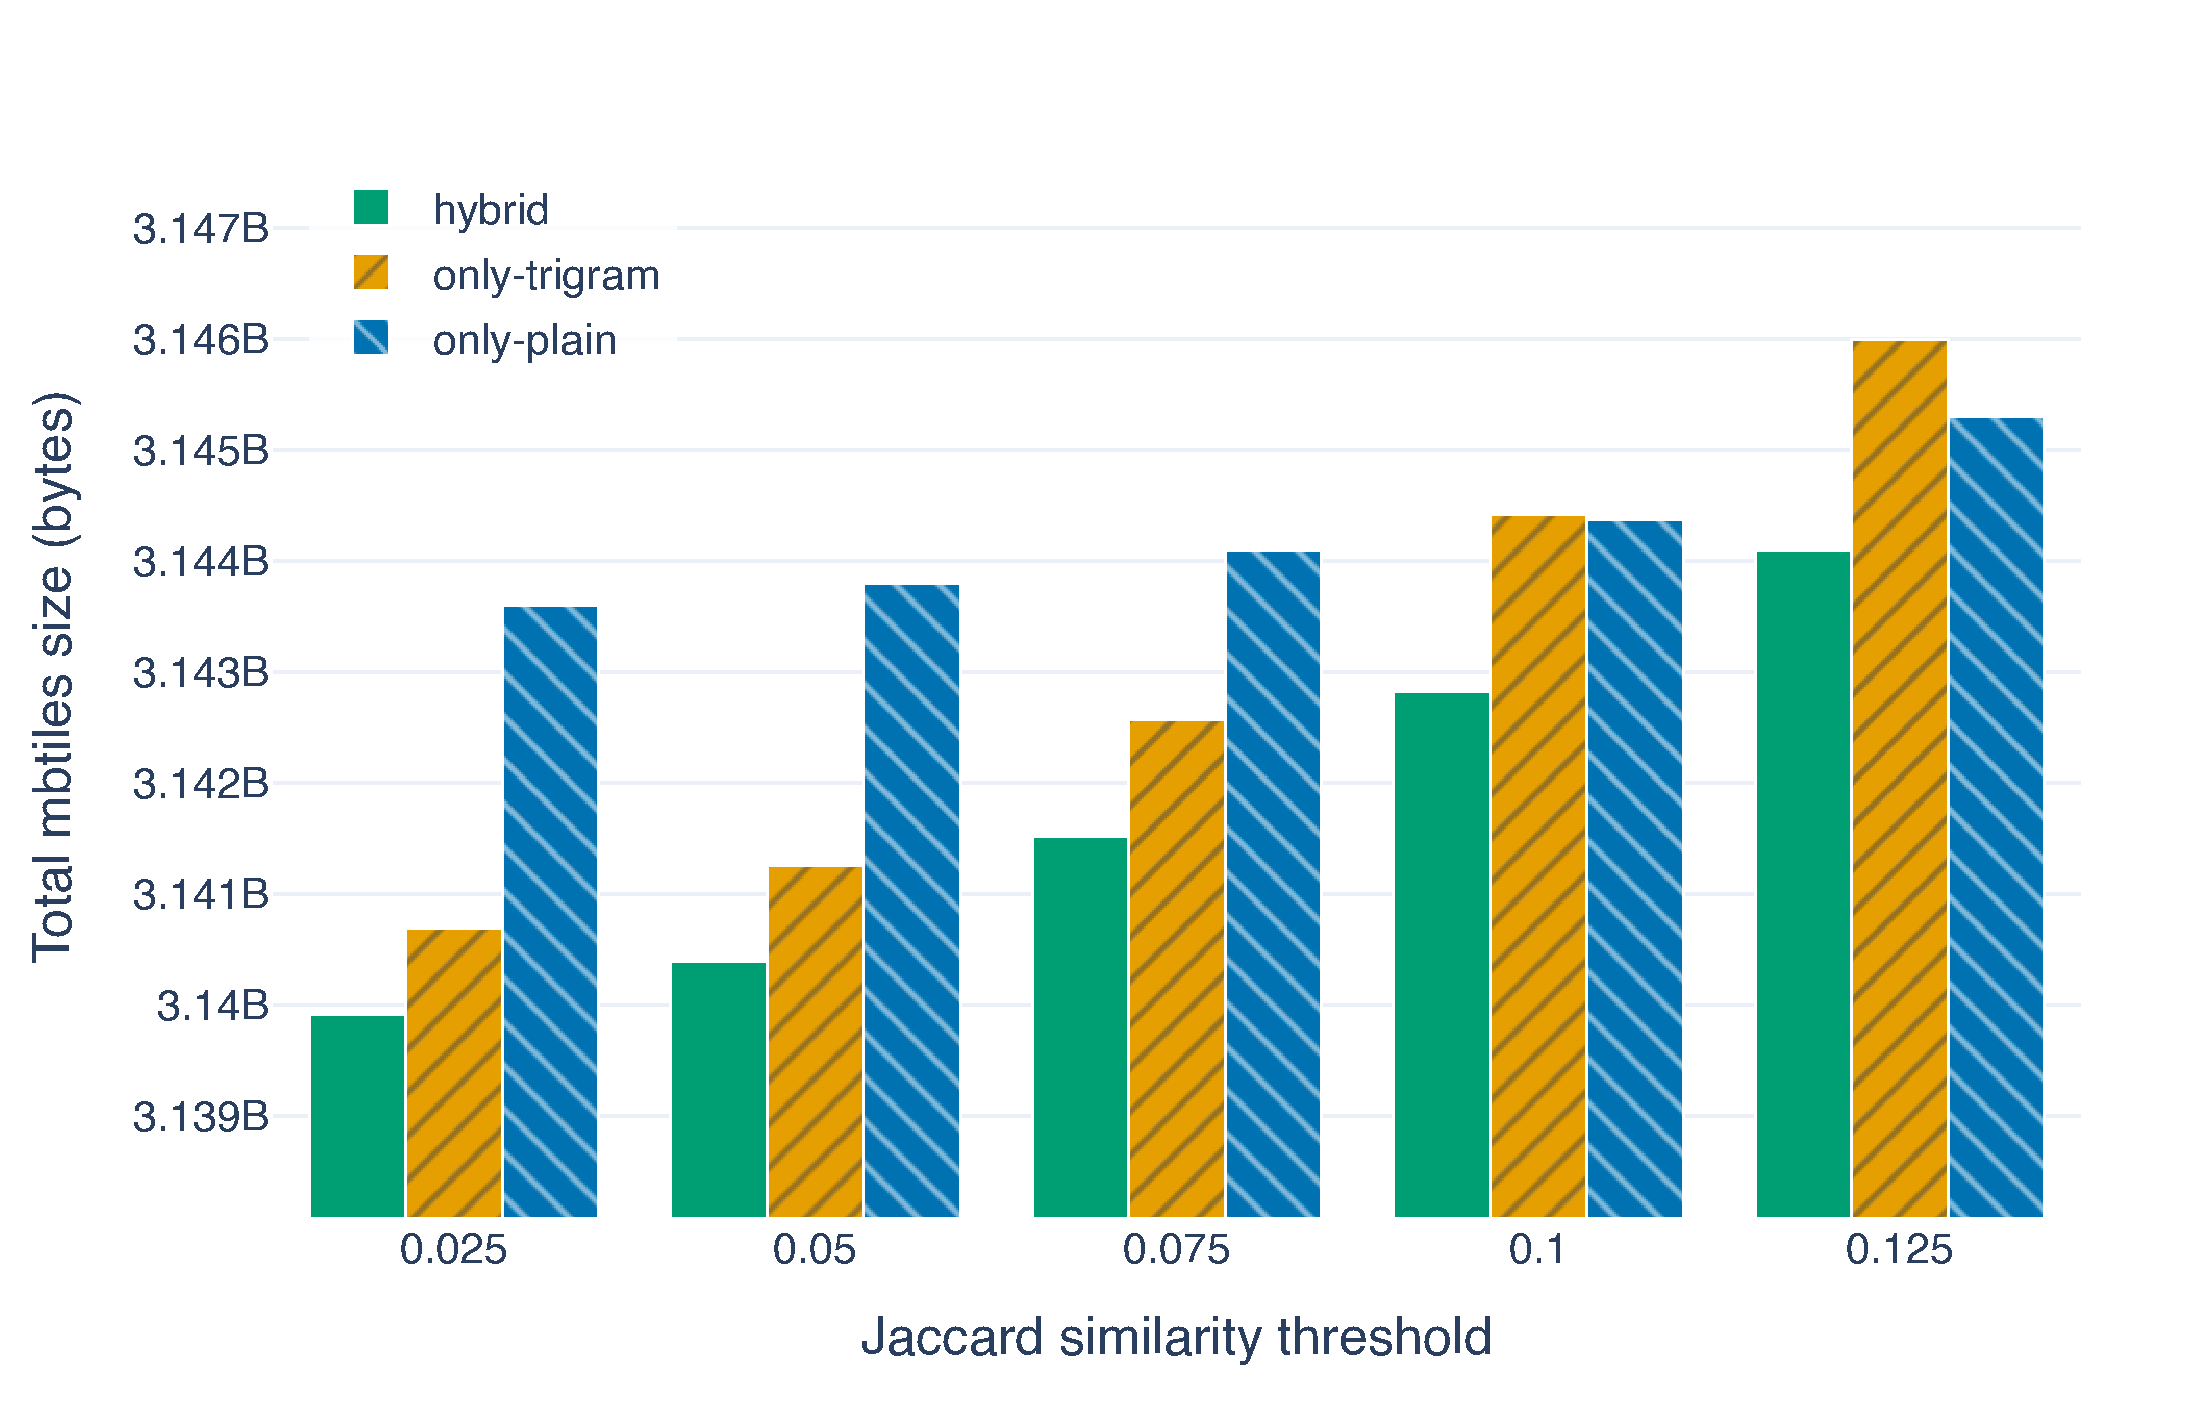
\includegraphics[width=0.8\linewidth]{figures/minhash_sweep.pdf}
    \caption{
Total encoded mbtiles size of the Germany OpenMapTiles tileset under different MinHash similarity modes and Jaccard thresholds.  Lower is better.  The hybrid mode (teal) produces the smallest output at every threshold.
All modes increase monotonically with threshold as fewer column pairs qualify for shared-dictionary grouping.
The y-axis is zoomed to the data range to make the differences visible: the full range spans approximately \qty{6}{\mega\byte} out of \qty{3.14}{\giga\byte} total}
    \label{fig:minhash_sweep}
\end{figure}